\section{Discussion: the mechanism of the recovery}\label{sec:discussion}

The scoring-face gain documented above invites a natural reading: the
contrastive-correctness adapter sharpens the model's internal direction for answer
correctness, so that cold multiple-choice scoring becomes more accurate. This
section shows the gain is better understood as a \emph{quantified causal
attribution} than as a sharpening. We take as established setup that cold
multiple-choice scoring under a chat template under-expresses knowledge the model
holds (\cref{sec:related}; \citealp{ConfidenceManifold,InsideOut,KAPPA}); the
result is what the adapter does about it. Most of the recovery is what
\emph{generic} fine-tuning buys (\cref{disc:inducibility}); it lives in a learned
direction that is off-axis-of-degree to the model's correctness geometry and is
causally privileged within that off-axis complement (\cref{disc:geometry}); it has
no layer locus (\cref{disc:locus}); and it does not transfer to generation
(\cref{disc:pathologies}).

The off-axis geometry is not a curiosity but the \emph{expected} signature of the
attribution we lead with, and reading it that way organizes the rest of this
section. The cold readout does not fail for lack of knowledge; it fails by
\textbf{surface-form swamping}: on the items the adapter fixes the base buries the
gold beneath more fluent distractors (\cref{disc:arbiter}). Plausibly, though we do
not measure this, suppressing surface form need not align with signalling
correctness. The two causal arms make the point in opposite directions: injecting
correctness \emph{on-axis} (the strongest on-axis reference we can build, $\Wknow$)
recovers only $\mathbf{6.4\%}$ of the lift, which refutes a knowledge-deficit
account; pushing \emph{off-axis} (perpendicular to correctness, $\offperp$) recovers
${\sim}$\textbf{100\%}, which is consistent with the surface-swamping account. The
off-axis direction is therefore not a spurious accident but a natural form for a
fix to take when the pathology is one of format rather than of knowledge --- which
is why a single off-axis push unifies the readout result (\cref{disc:arbiter}), the
inducibility attribution (\cref{disc:inducibility}), the on-axis null
(\cref{disc:geometry}), and the deployment pathologies (\cref{disc:pathologies}).

\subsection{The fixed items are chain-of-thought-accessible, the no-transfer is
out-of-task (not difficulty-bound), and the readout misranks by confident burial}
\label{disc:arbiter}

The cleanest evidence that the readout --- not the model's knowledge --- is the
bottleneck comes from a per-item arbiter. We isolate the \textbf{124} ARC items the
adapter corrects in cold multiple-choice scoring but the on-axis offset does not
(\cref{disc:geometry}), and for each ask whether the \emph{base} model already
reaches the right answer through generative chain-of-thought. It does: the base
solves $\mathbf{124/124}$ ($1.000$) of these items under generative CoT (the
fixed-parser re-run resolves the earlier 123/124: the one ``failure'' was a parser
artifact --- doc 128's numeric option label ``4'', which the letter-parser could not
emit by construction --- now parsing correct, n\_unparsed $5{\rightarrow}0$),
indistinguishable from its CoT accuracy on the items it already scores correctly
cold (base-right control, $200/202 = 0.990$ --- read from the same fixed-parser run,
not from the superseded pre-fix one, where it was 196/202). The items the adapter
``fixes'' are knowledge the base already reaches by reasoning; cold scoring simply
misranks them.

\paragraph{The arbiter discriminates: a negative control on the adapter's
residual.}
A per-item arbiter of this shape invites an obvious objection --- if the base
solved \emph{everything} under chain-of-thought, ``the fixed items were already
CoT-accessible'' would be true of all of ARC and would say nothing about the
adapter. The control is the complementary population, and it needs no new
generation: the v2 arbiter run already covers all 400 items under the identical
protocol (greedy $k{=}1$, same prompt, same fixed parser, \code{n\_\allowbreak unparsed=0}), so
re-partitioning it is protocol-identical to the headline by construction. On the
adapter's \textbf{residual} --- the 47 base-wrong items it does not fix --- the base
solves $\mathbf{41/47 = 0.872}$ (CI $[0.748, 0.940]$), against $\mathbf{151/151}$ on
the base-wrong items it does fix (Fisher $p=1.4\times10^{-4}$) and
$\mathbf{392/400 = 0.980}$ over all of ARC ($p=0.0015$). A related partition in the
independent premise-file scaffold --- which defines the $n{=}73$ residual of the PMI
residual-discrimination analysis below; the calibration analysis runs on the lm-eval
scaffold --- agrees: $66/73 = 0.904$ against $326/327 = 0.997$,
$p=3.6\times10^{-5}$. It is \emph{related} rather than identical, and we say so: the
lm-eval partition conditions on base-wrong (47 against 151), while the $n{=}73$ is
every item the adapter gets wrong, including 8 it broke from base-right. Restricting
it to base-wrong for a like-for-like read gives $58/65 = 0.892$, between the two. So
the 124/124 is not trivially true of all of ARC. Two honest qualifications travel
with it. First, the magnitude is modest in absolute terms --- ARC is near its CoT
ceiling everywhere, and the discrimination is 0.872 against 0.980, not against
something far lower. Second, the residual figure fell \emph{between} the two
thresholds we pre-registered for this control (${\leq}0.85$ $\rightarrow$
discriminates, ${\approx}0.97$ $\rightarrow$ saturated); we therefore rest the
reading on the contrast and its interval (CI upper 0.940 excludes the saturated
value) rather than on the point estimate clearing a bar it did not clear. The
adapter is a \emph{shortcut} to that knowledge --- it nudges the scoring logits
toward answers the base could reason its way to, without reasoning.

This directly explains why the lift does not transfer to generation
(\cref{sec:results}): on exactly these items the base is already at ceiling under
CoT, so there is no generative headroom for a scoring shortcut to add. The obvious
objection is that ARC is simply easy --- near its CoT ceiling --- so the arbiter
cannot tell ``recovers knowable'' from ``fabricates plausible.'' We corroborate the
no-transfer out-of-task.

On \textbf{GPQA}, where the base must genuinely reason, its CoT accuracy is
$\mathbf{0.7071}$ (arbiter; 140/198, thinking-on, with the generation budget raised
to 8192 tokens --- at 2048 the base truncated 96\% of its reasoning, producing a
spurious 0.15). Two things follow. First, 0.7071 is well above chance, so the base
\emph{does} solve these by reasoning; yet the cold-scoring shortcut still has no
generative headroom to add, and indeed the measured cold-MC lift on GPQA is
${\sim}0$ (base $0.4747 \rightarrow$ adapter $0.4697$, $-0.5\pp$, CI crossing zero)
--- the no-transfer result restated out-of-task. This is a
no-transfer-\emph{out-of-task} result, not a no-transfer-to-\emph{hard} one: GPQA is
out-of-task and distribution-distant (it is the B.2 spillover task at $-6.6\pp$).
Second, because the base already reasons GPQA out, a verifier-guided arm (base
generates, adapter scores) has nothing to harvest, so we did not build one (a design
choice following from the result, not an independent test). The
readout-is-the-bottleneck result therefore survives an out-of-task control that the
ARC arbiter alone could not provide.

Two added controls now separate difficulty from distribution, where previously a
single out-of-task benchmark could not. \emph{Within-format difficulty:} the cold-MC
fix-rate on base-wrong items moves only $\mathbf{-0.10}$ as ARC difficulty rises
(ARC-Easy 0.861, $n{=}360$ $\rightarrow$ ARC-Challenge 0.763, $n{=}198$, both
burial-matched by gold-rank), whereas it collapses $\mathbf{-0.56}$ going
out-of-task to GPQA (0.202) --- so \emph{distribution}, not within-format
difficulty, drives the collapse. \emph{A second pair of anchors:} on HellaSwag and
Winogrande, where the lift also holds ($+17$ / $+19$), the base's CoT accuracy is
high (0.83 / 0.9425) --- like ARC's 0.97 and well above GPQA's 0.70 --- and the
recovery is recoverability-gated (the adapter fixes CoT-right items more than
CoT-wrong ones: HellaSwag 0.64 vs 0.31, Winogrande 0.76 vs 0.42), i.e.\ the lift
rescues knowledge the base can already reason out. The no-transfer is therefore
\textbf{out-of-task, not difficulty-bound} --- supported now, not merely
suggestive, on all three anchors. \emph{(Power caveat: the hard cells are small ---
HellaSwag $n{=}32$, Winogrande $n{=}12$ --- and the Easy${\rightarrow}$Challenge
difficulty range stays below GPQA's, both base-CoT near 0.97; the burial gradient is
shallow throughout, corr(fix, z-gap) $-0.17$.)}

\paragraph{How the readout misranks on ARC: confident burial under fluency.}
The arbiter shows the model \emph{has} the answer; a calibration analysis on ARC
shows \emph{how} cold scoring loses it, and it is not indifference between close
options but misplaced confidence. We measure this on an \textbf{adapter-independent}
subset --- the $n{=}192$ ARC items the base scores wrong cold yet solves under CoT
($S_{\mathrm{cot\_coldwrong}}$, defined without any reference to the adapter) --- so
the signature cannot be an artifact of which items the adapter happened to fix. On
these items the base's chosen (wrong) option beats the gold by $\mathbf{1.45\sigma}$
within-item, the gold sits at \textbf{median rank 2 of 4} (only 41\% have the gold
at rank 1), and a gold-vs-distractor ranking on the base-wrong items scores
\textbf{AUC 0.394, \emph{below} chance}. (This confident-wrong signature is the
multiple-choice overconfidence aligned-model calibration work documents, which
separates an \emph{answer-decision} uncertainty from a \emph{format-preference}
uncertainty and attributes alignment overconfidence to their conflation
\citep{AlignedMCCalibration}; our claim goes past calibration --- the per-item
arbiter shows the buried answer is \emph{reachable}, at 124/124 under CoT, and a
learned offset \emph{exploits} the gap rather than re-calibrating it post hoc.) The
gold is not a flat near-miss; it is actively \emph{buried} beneath more fluent
surface forms --- the base's raw pick is the gold only \textbf{19\%} of the time
here, against \textbf{81\%} on the items it scores correctly cold.

The re-ranking the adapter performs is \textbf{promotion-dominated} (it adds 0.35 of
probability mass to the gold while removing 0.21 from wrong options, and sharpens
the distribution, $\Delta$entropy $-0.19$), consistent with surfacing a
buried-but-present signal rather than manufacturing one.

\emph{Methodological note we are forced to make:} the apparent \emph{flatness} of
the char-normalized answer entropy (0.920 on this subset) is a softmax-temperature
artifact --- length normalization compresses the spread ${\sim}50\times$ without
reordering, while the raw distribution is peaked. We therefore report \textbf{rank
and within-item z-gap}, which are invariant to that normalization, and not entropy,
whose flatness flips with the metric. (The selection-conditioned
$S_{\mathrm{flip}}$ subset, the 151 items the adapter flips, shows the identical
signature --- z-gap $1.37\sigma$, gold-rank median 2 --- and serves only as a
consistency check; its conditioning on the adapter's flips is why the
adapter-independent subset is the headline.)

This burial-and-recoverability signature is established on ARC; we \textbf{could not
detect} it out-of-task on GPQA, but as a power-starved non-finding rather than a
contrast: on the burial-matched hard cell the CoT-right and CoT-wrong fix-rates are
equal ($0.186 = 0.186$), but $n{=}43$ with 31 items left unparsed ($k{=}1$ greedy
decoding) contaminates that cell, leaving it indistinguishable from no measurement.
We therefore report the recoverability-gating as \textbf{could-not-detect /
power-starved out-of-task}, not as evidence against it.

\paragraph{The signal is swamped, not absent --- ``broken'' means \emph{lossy}.}
It does not follow that the cold channel is empty. After removing length and fluency
(a PMI / decision-conditional residual), a gold-vs-distractor discrimination scores
above chance on both arms in the \emph{same scalar channel}: \textbf{AUC 0.574} (CI
$[0.520, 0.627]$) on the base-wrong items ($n{=}204$), and \textbf{0.667} (CI
$[0.584, 0.744]$) on the adapter's own residual ($n{=}73$, the items it does not
fix). The correctness signal is present in the cold channel but \emph{out-ranked} by
fluency, not erased: the same PMI-residual channel carries gold-vs-distractor
signal, rather than the channel being empty and the adapter supplying missing
knowledge.

\emph{Honesty boundary:} these are two arm readings on \textbf{different
populations} ($n{=}204$ vs $n{=}73$), not a within-set rise; and the base-arm CI
lower bound, 0.520, does not on its own clear a 0.55 ``present'' threshold --- we
call the base channel \emph{intermediate} and rest the present-but-swamped claim on
the adapter arm (CI lower bound $0.584 > 0.55$), and raising power on the base arm
did not rescue it: pooling base-wrong with $S_{\mathrm{cot\_coldwrong}}$ --- and
every defensible pool variant --- ran, and none clears 0.55. The
adapter-independent $S_{\mathrm{cot\_coldwrong}}$ ($n{=}192$, the items the base
\emph{provably} knows via CoT yet cold-MC misranks) reaches only CI lower bound
0.512, and even the literal union base-wrong ${\cup}$ $S_{\mathrm{cot\_coldwrong}}$
($n{=}228$, which is \emph{pro}-gate --- its 24 extra items are base-right under
premise scoring) reaches 0.535, so the base channel stays \emph{intermediate} on the
strongest honest pool.

\subsection{Much of the recovery is generic to fine-tuning; how much depends on
capacity and on the task}\label{disc:inducibility}

If the lift were a specific consequence of the \emph{contrastive-correctness}
objective, an ordinary supervised fine-tune should not reproduce it. It largely does
--- and running the control at two very different capacities shows that ``how much''
is not a single number.

\textbf{At the adapter's own capacity.} The same-parameterization control
(\cref{method:neteffect}: identical 48 head-pairs, identical $12{,}336$ trainable
parameters, identical corpus/steps/split/checkpoint rule, ordinary cross-entropy on
the correct answer only, three seeds) recovers $\mathbf{36.2\% \pm 5.0}$ of the ARC
lift, or $39.7\% \pm 3.1$ if the fixed final step is used instead of the
best-validation checkpoint --- a ${\sim}36$--$40\%$ range. Because the intervention
space is held exactly fixed here, this is the arm that attributes recovery to the
objective as such.

\textbf{At $1{,}800\times$--$58{,}000\times$ capacity.} A non-contrastive Align-LoRA
on the same data budget, run through the same causal recovery machinery (a sign-safe
three-zone control gate), recovers about \textbf{62\%} of the ARC lift, and that
fraction is \textbf{flat across a rank sweep} (r8/32/64/256: 59/63/60/65), with the
sweep slope's confidence interval spanning zero ($[-1.4, +3.4]$) and a
paired-bootstrap fraction interval of $\mathbf{[51\%, 73\%]}$. That interval resamples
the $400$ items with replacement and carries the base, generic and contrastive arms
together, so the positive inter-arm correlation the three arms actually have
(item-level $r{=}0.42$ between base and generic) is retained instead of discarded; it
is $44\%$ narrower than, and contained in, the delta-method $[45\%, 85\%]$ we report
as the conservative reading (zone C is binned on the point estimate, $0.62$, and is
unchanged). One-sided, the fraction exceeds one half in $98.2\%$ of resamples --- one
minus the one-sided bootstrap $p$-value, not a posterior probability. Under raw
accuracy instead of length-normalised accuracy the point moves to $0.61$ and that
figure to $96.9\%$. Within that grid, then, the
residual is not a gap more rank closes; but the comparison with the
same-parameterization arm shows that capacity itself moves the fraction, from
${\sim}37\%$ to ${\sim}62\%$. We therefore do not name a ceiling for generic
fine-tuning, and we treat the contrastive-specific residual as \emph{grid-relative}:
${\sim}60$--$64\%$ of the ARC lift at equal capacity, ${\sim}38\%$ against the
higher-capacity arm.

One caveat we apply to ourselves, symmetric with the information-set discipline of
\cref{disc:channel}: matching examples and optimizer steps does not match the
effective training signal per step --- the contrastive objective sees each example
with an explicit correct/incorrect contrast where the plain objective sees only the
correct completion --- so these fractions attribute the lift to \emph{fine-tuning on
this data} rather than to any stronger claim of per-step informational equivalence.
Indeed the task breakdown suggests that contrast is exactly what the harder cases
need: the same three same-parameterization seeds recover $79.5\% \pm 1.4$ of the
Winogrande lift and $69.5\% \pm 6.4$ of HellaSwag's --- where scoring rewards the
plausibility of a continuation --- but $0.9\% \pm 3.3$ of TruthfulQA-mc1's, where a
plausible distractor must be beaten, despite TruthfulQA sitting in the control's own
training corpus. ARC, at ${\sim}37\%$, falls between the two regimes.

We restrict this control to ARC because TruthfulQA's matched corpus leaks into its
evaluation. Across the rank sweep the TQA recovered fraction rises monotonically
(41/66/72/91), the signature of memorizing training examples that recur at test;
held out on 20\% of TQA, the highest-rank control collapses from 98\% to 30\%
recovery and the rank sweep flattens (r8 = r256 = 0.524), while the contrastive
adapter still generalizes held-out (0.83). The matched corpus (TQA train-80\%, seed
0) overlaps the evaluation set; TQA is therefore excluded from the inducibility
control, and the ${\sim}62\%$ generic figure is an ARC result.

\subsection{The lift does not reduce to an interpretable re-scoring of the output
scalars}\label{disc:channel}

The inducibility result attributes most of the lift to generic fine-tuning, but it
leaves a sharper question: whether the recovered signal is a simple, interpretable
re-weighting of the scores the cold readout already produces (length, PMI, an
answer prior, a calibration temperature). If so, the ``lost'' knowledge would be
recoverable by post-hoc re-scoring alone, without touching the model's activations.
It is not. We build the strongest such re-scorer we can --- a supervised, held-out,
AUC-objective combination of the interpretable surface features (conditional
log-likelihood, answer-only log-likelihood, character length, PMI) --- and ask how
well it separates gold from distractor on the base-wrong items. It caps at
\textbf{AUC 0.574} (a held-out logistic fit at 0.458 and a non-linear GBM at 0.462,
an on-test-tuned oracle stack at 0.502, PMI alone at 0.574), against the
\textbf{adapter's 0.830} on the same items. PMI does not merely fail to match the
adapter --- applied \emph{to} the adapter it \emph{hurts} it
($0.818 \rightarrow 0.758$), and the adapter's re-ranking is only \textbf{2.4\%}
explained by the surface features ($R^2$ 0.024). The recovered signal therefore
lives \textbf{upstream of the collapsed output scalars}: no re-scoring of those
scalars recovers the lift, which answers the ``your baseline is just under-fit''
objection --- the ceiling is supervised and held-out, not a hand-tuned stack.

We are deliberate about what this licenses. The comparison is
\emph{information-set-confounded} --- the adapter mutates \textbf{activations},
whereas the surface stack re-weights \textbf{collapsed output scalars} --- so the
gap (0.830 vs 0.574) does \textbf{not} license ``a magic off-axis direction'' (a
generic SFT recovers ${\sim}62\%$ the same way, \cref{disc:inducibility}) nor ``an
empty channel'' (the residual is $0.574 >$ chance, \cref{disc:arbiter}). The
defensible claim is about the \textbf{channel}: the lossy readout discards signal
that survives in the activations and is not reconstructible from its own outputs.

We can now sharpen the channel claim with a same-space probe. A logistic probe fit
on the \emph{same} per-head \code{o\_\allowbreak proj}-input activations the adapter writes to
--- no fine-tuning, held out by item, on the same cold-MC option-continuation
distribution, scaler${\rightarrow}$PCA${\rightarrow}$logistic with the preprocessing
fit inside each fold and a within-item label-permutation null --- recovers
gold-vs-distractor on ARC base-wrong items at \textbf{AUC 0.955} (CI
$[0.934, 0.973]$, permutation null 0.494), far above the \textbf{0.502}
collapsed-output ceiling. A surface-form control --- the same probe on length/format
features of the option string --- caps at \textbf{0.442} (${\approx}$ chance), so
the 0.955 reads correctness the output scalars discard, not a length/format
artifact. This \textbf{widens and cleans the channel gap}
($0.502{\rightarrow}0.955$) relative to the scalar-stack version
($0.574{\rightarrow}0.830$).

We are careful about what it does \textbf{not} license. First, the probe reads
12288 activation dimensions while the adapter is constrained to nudge output logits.
The two are not on the same axis, so 0.955 is \textbf{not} ``the probe beats the
adapter,'' and we do not read it as a representational \emph{edit}. Second, that a
linear probe decodes correctness from activations at ${\sim}0.95$ is a
near-universal property of capable language models
\citep{AzariaMitchell,MarksTegmark}. It shows the information \emph{exists} in the
activations the readout collapses, \textbf{not} that the model's own deployed
readout is ``merely miscalibrated.'' We therefore make a \textbf{sharpened channel
claim} --- the cold-MC output-scalar channel is lossy relative to the activation
channel --- and we do \textbf{not} assert ``pure miscalibration'' or ``signal intact
upstream'' as anything beyond that channel statement.

Third, the recoverable signal is \textbf{broadly distributed}: a random 48-head set
decodes it as well (0.949 ${\approx}$ the adapter's 48 heads), so the probe speaks
to the cold-MC channel being lossy \emph{model-wide}, not to the adapter's subspace
being privileged. This is a read-test about the channel, decoupled from the
write-tests that establish the adapter's specificity (a random norm-matched
\emph{offset} recovers ${\sim}0\%$ of the \emph{lift}, \cref{disc:geometry}, a
different operation). On TruthfulQA the same probe reaches 0.974, but its
surface-form control is non-trivial (0.639, with a gold-first position artifact at
1.000), consistent with TruthfulQA's answer-prior character
(\cref{disc:heterogeneity}); the channel claim is therefore anchored on ARC.

\subsection{A read-only selector deploys the recovered signal without the
pathologies}\label{disc:selector}

The channel result has a constructive consequence --- but we scope it as the
\emph{read leg of a read${\neq}$write dissociation}, not as a new method, because
the bare capability is already published. That a read-only probe or readout can
\emph{select} multiple-choice answers and recover an accuracy lift, with no weight
edit and no generation, is established by at least two independent mechanisms: NoVo
selects answers by voting over truth-correlated attention-head norms ($+19$ points
on TruthfulQA-MC1, gains on ${>}90\%$ of 20 datasets) \citep{NoVo}, and CORAL
re-scores per-option probabilities with a frozen weight-decay correctness probe
($+14\%$ accuracy on ARC-Challenge/HellaSwag/OpenBookQA/Math-MC, 7B models)
\citep{CORAL}. Both present the selector as a calibration/accuracy \emph{fix}; our
use is narrower and different --- the read-only selector is the \emph{evidence} that
the lift the adapter writes off-axis is recoverable read-only, on-axis, without the
write's damage (a read${\neq}$write dissociation neither studies, lacking an
off-axis adapter to audit). If the correctness signal the cold readout discards is
\emph{present and read-only recoverable} in the activations, then one can recover
the MC lift without writing any offset at all --- and therefore without the
deployment pathologies the write incurs (\cref{disc:pathologies}).

We deploy the same-space probe of \cref{disc:channel} as a \textbf{read-only
selector}: for each cold-MC item it reads the per-head activations and picks the
option the probe scores highest, with no offset injected and no change to
generation. On ARC it reaches selector accuracy \textbf{0.943} ($\pm$ 0.002 over
three seeds), against the base's 0.505 and the adapter's 0.853, and the gain is not
a correct-for-wrong trade: relative to the base it fixes \textbf{181} of the 198
base-wrong items and breaks only \textbf{5} of the 202 base-right ones (exact
McNemar $p = 3.7\times10^{-47}$; an accuracy-space permutation null sits at 0.255).
Because it never touches the weights or the decoder, it carries none of the
adapter's costs --- no retrieval spillover, no generation loss (no reasoning
breakage) --- so on the (cost, MC-accuracy) plane it \textbf{Pareto-dominates the
adapter}. Whether it also wins on deployment grounds --- against the
\emph{reasoning} baseline the no-headroom arbiter (\cref{disc:arbiter}, base
124/124 under CoT) suggests, and against the trivial one-forward baseline --- is
settled below by the deployment triangle: it does \textbf{not}. A
reasoning TTC ties the cheapest baseline, and a single-forward letter-emission of
the base dominates the selector outright, at \emph{half} its measured cost --- which
is exactly why we hold the selector to its \emph{evidentiary} role
(read${\neq}$write) rather than a deployment win.

We hold the claim to its read side and guard against an over-reading: 0.943
exceeding the adapter's 0.853 is \textbf{not} ``the probe beats the adapter as a
capability'' --- the probe reads 12288 activation dimensions while the adapter is
constrained to nudge collapsed output logits, so the two are not on the same axis
(\cref{disc:channel}). The claim is that the cold-MC channel \emph{discards} a
signal a linear reader recovers read-only. One caveat bounds the contribution to
Tier-1: the 48-cell feature set is held out by \emph{item} but selected on the
training split, not held out by \emph{feature}, so the decisive strengthening is
cross-benchmark (ARC-Easy / OpenBookQA), which we flag as the immediate follow-up.

\paragraph{The deployment triangle (\cref{fig:triangle}).}
The read-only selector is neither the strongest nor the cheapest good way to answer
these items --- both distinctions belong to the base model asked correctly. On the
198 base-wrong ARC items we benchmarked four deployment routes on one homogeneous
cost unit: median (p50) end-to-end latency per item at batch~1 on an RTX PRO 6000
(bf16), reported alongside the tokens each route actually consumes
(\cref{tab:triangle}). This matters because ``one forward'' is not one unit of work:
cold-MC scoring and the selector must score \emph{every option continuation}
separately (${\sim}4$ per ARC item, ${\sim}24.7$ scored continuation tokens), whereas
letter emission is a single forward plus two generated tokens.

Measured, the routes are: the contrastive adapter's cold-MC scoring recovers
\textbf{0.757} at \textbf{354\,ms}; the read-only selector \textbf{0.911} at
\textbf{360\,ms}; prompting the base to emit the answer letter in one greedy forward,
no chain of thought, recovers \textbf{0.970} (192/198; 2 items unparsed and counted
wrong, so a floor) at \textbf{181\,ms}; and a reasoning test-time-compute baseline
(base self-consistency CoT, $k{=}3$) also recovers \textbf{0.970}, at
\textbf{26.7\,s} and $853.9$ generated tokens summed over its three traces. So letter
emission is not merely a same-cost tie --- it is the \emph{cheapest and the most
accurate} route on the plane: it costs about half what the adapter and the selector
cost, beats the adapter by $21$ points and the selector by $6$, and matches the
reasoning baseline at ${\sim}150\times$ less latency. The adapter is dominated by
every other route, including on cost.

One caveat scopes this exactly as it scopes the arbiter (\cref{method:protocol}):
letter emission puts the base in a lettered-MCQ format, a \emph{different readout}
from the cold-MC option-continuation scoring the adapter operates on --- not a
like-for-like scoring comparison. That is the point rather than a confound: it
compares two readouts of the \emph{same base} --- loglik continuation ranking vs
letter emission --- which move it from 0.505 to 0.980 over the full set
($0{\rightarrow}0.970$ on the base-wrong subset the triangle uses), with the cheaper
readout winning. This is the paper's thesis, that the cold-MC channel is lossy, in
its sharpest form: the knowledge is present and cheaply reachable by a different
readout of the base, and the adapter's off-axis write recovers \emph{less} of it
(0.757) than the most trivial alternative does for less money (0.970).

\begin{figure}[t]
\centering
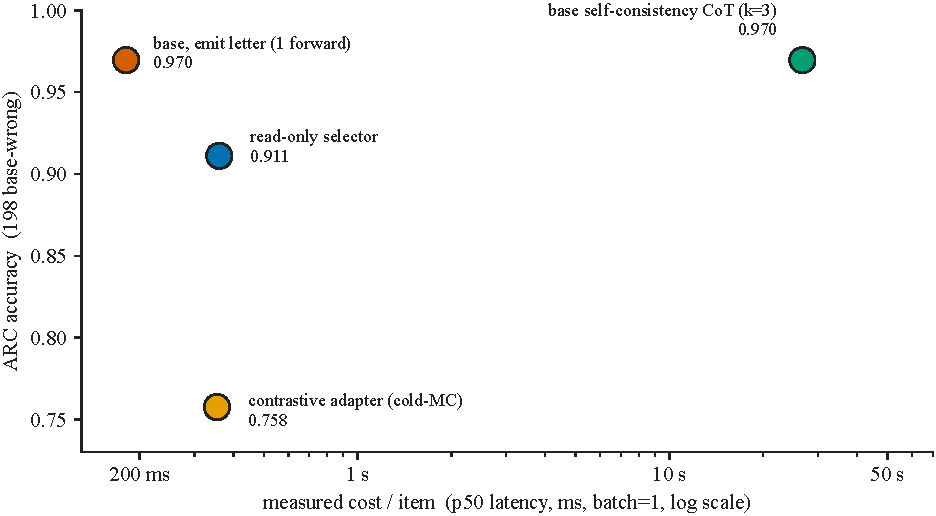
\includegraphics[width=.78\textwidth,alt={Scatter plot of the deployment triangle
on the 198 base-wrong ARC items: x-axis is measured median per-item latency at batch
one on a log scale, y-axis is ARC accuracy. Base letter-emission is the top-left
point at 0.970 accuracy and 181 milliseconds; the read-only selector sits at 0.911
and 360 milliseconds; the contrastive adapter at 0.757 and 354 milliseconds; base
self-consistency chain-of-thought far to the right at 0.970 and 26.7
seconds.}]{figures/fig_deployment_triangle.pdf}
\caption{\textbf{The deployment triangle on the 198 base-wrong ARC items, on measured
cost.} $x$: median (p50) per-item latency at batch~1, bf16, RTX PRO 6000 (log scale);
$y$: ARC accuracy. One homogeneous unit for all four routes, replacing the earlier
mixed forwards/tokens proxy --- ``one forward'' is not one unit of work, since cold-MC
scoring and the selector score every option continuation separately (${\sim}4$ per
item) while letter emission is one forward plus two tokens. Four routes: the
contrastive adapter's cold-MC scoring (0.757, 354\,ms) is dominated by everything, on
accuracy \emph{and} on cost; the read-only selector (0.911, 360\,ms) improves on it
read-only; \textbf{the base asked to emit the answer letter in one forward (0.970,
181\,ms) is both the cheapest and the most accurate route --- it matches the reasoning
baseline at ${\sim}150\times$ less latency and strictly dominates the adapter and the
selector at about half their cost}; base self-consistency CoT (0.970, 26.7\,s, 853.9
generated tokens over three traces) ties letter emission at far higher cost. The whole
LoFiT/ITI-for-cold-MC family optimizes a readout that the most trivial and cheapest
alternative --- ask the base for the letter --- already beats. \textbf{The comparison
is evidentiary, not a like-for-like scoring test:} letter emission is a different
(lettered-MCQ) readout than the cold-MC channel (\cref{method:protocol}), so the
triangle contrasts two readouts of the same base --- the lossy-readout thesis in its
sharpest form --- and the selector's role stays evidentiary (read${\neq}$write), not a
deployment recommendation, since even it is dominated by letter emission. Cost is
latency on this one accelerator at batch~1; we do not normalize FLOPs across readouts,
and batched throughput (reported in \cref{tab:triangle}) is not comparable between
prefill-bound scoring and decode-bound generation.}
\label{fig:triangle}
\end{figure}

\begin{table}[tbp]
\centering
\begin{threeparttable}
\caption{\textbf{Deployment routes on the 198 base-wrong ARC items, measured cost}
(the numeric view of \cref{fig:triangle}). Latency is median (p50) / 95th percentile
per item at batch~1, bf16, single RTX PRO 6000; tokens are generated tokens for the
generation routes and scored continuation tokens for the scoring routes. Batched
throughput is listed for completeness but is \emph{not} comparable across route
families (prefill-bound scoring vs decode-bound generation).}
\label{tab:triangle}
\footnotesize
\begin{tabular}{L{3.5cm} L{3.1cm} L{2.5cm} L{1.9cm} L{2.9cm}}
\toprule
Deployment route & ARC accuracy (198 base-wrong) & Latency p50 / p95 & Tokens /
item & Relation \\
\midrule
\textbf{Base letter-emission (1 forward, no CoT)} & \textbf{0.970} (192/198; 2
unparsed as wrong $\rightarrow$ floor) & \textbf{181 / 253\,ms} & 2.0 generated &
\textbf{cheapest \emph{and} most accurate: matches SC-CoT, strictly dominates
selector and adapter} \\
Base self-consistency CoT ($k{=}3$) & \textbf{0.970} (192/198; $k{=}5$ identical
$\rightarrow$ saturates at $k{=}3$) & 26.7 / 36.6\,s & 853.9 generated (sum over
3 traces) & ties letter-emission at ${\sim}150\times$ the latency \\
Read-only selector (\cref{disc:selector}) & \textbf{0.911} (5 probe seeds) & 360 /
479\,ms & 24.7 scored (${\sim}4$ options) & dominated by letter-emission (2$\times$
its cost, $-6$pp); Pareto-dominates only the \emph{adapter} \\
Contrastive adapter (cold-MC scoring) & \textbf{0.757} & 354 / 471\,ms & 24.7 scored
(${\sim}4$ options) & dominated by all three, on accuracy \emph{and} cost \\
\bottomrule
\end{tabular}
\begin{tablenotes}[flushleft]\footnotesize
\item \textbf{Provenance and one reconciliation.} Measured in a single harness that
re-derives every route's per-item correctness and validates it against the canonical
lm-eval artifacts before timing (\code{runs/\allowbreak e3\_\allowbreak cost/}). Within that harness the
adapter scores $0.757$ (150/198) and the base cold-MC arm $0.5025$, against $0.7626$
(151/198) and $0.5050$ in lm-eval: a one-item difference in both arms, from the
context/continuation tokenisation boundary in the re-implemented log-likelihood. The
canonical accuracies elsewhere in this paper are the lm-eval ones; the $0.757$ here is
the number produced by the same code path that produced the latencies, which is why we
report it in this table rather than silently mixing sources.
\end{tablenotes}
\end{threeparttable}
\end{table}

The selector Pareto-dominates only the \emph{adapter}; a reasoning TTC and a
one-forward letter-emission of the base both beat it --- so the whole
LoFiT/ITI-for-cold-MC family optimizes a readout that even asking the base for the
letter already beats. We therefore report the selector as \emph{evidentiary} (the
correctness signal is read-only recoverable, read${\neq}$write) and \textbf{not} as
a deployment win (dominated by letter emission at half its measured cost).
\emph{Population note (do not conflate):} the four figures here (letter-emission
0.970, SC-CoT 0.970, selector 0.911, adapter 0.757) are all on the \textbf{198
base-wrong}
subset; the selector's all-items accuracy (\textbf{0.943}, three seeds, across all
$n{=}400$ evaluation items) and the adapter's all-items accuracy
(\textbf{0.853/0.855}; \cref{tab:headline}) are computed on a \emph{different}
population and are not directly comparable to the 0.911 / 0.757 here. The 0.943 and
0.911 are the same selector on two populations, not two systems (and the canonical
lm-eval value on this subset is 0.914; the 0.911 is the same selector re-fit inside the
cost harness, see the table note). ``All items'' here
means the $n{=}400$ harness sample, \textbf{not} the full ARC-Challenge test split
--- that phrase is reserved for the R4 full-split run (\cref{sec:limitations}, ARC
acc\_norm $+36.2$).

\paragraph{read ${\neq}$ write, geometrically.}
The selector and the off-axis write together make a four-way dissociation the paper
rests on. A reader \emph{reads} correctness from the activations (selector 0.943);
an \emph{on-axis} write fails to recover the lift ($\Wknow$ 6.4\%); an
\emph{off-axis} write succeeds ($\offperp$ ${\sim}100\%$, shuffle ${\sim}0\%$,
\cref{disc:geometry}); and --- closing the loop --- the probe's decision direction
is geometrically aligned with the correctness axis it reads, \emph{not} with the
axis the adapter writes. Per head, the probe direction's signed cosine with the
functional correctness direction $\vinf$ is $+0.22$ (median $+0.20$, above the
${\sim}0.06$ null band), while its cosine with the adapter's write direction
$\thetamc$ is $|0.066|$ (at the edge of the ${\sim}0.061$ per-head null band, not
clearly within); pooled, $+0.209$ vs $|0.008|$ (clearly within the null --- the
read${\neq}$write conclusion rests on the pooled statistic). The read axis is
$\vinf$; the write axis is off-axis to it. We mark this geometric leg
\textbf{moderate, not a slam-dunk}: the alignment is 0.22 rather than 0.5,
fold-stability is 0.887 (marginal at $n \ll d = 12288$), and $\vinf$ lives strongly
on the top principal component (cos 0.55) --- but the probe reads $\vinf$ 66\%
\emph{beyond} PC1 (its PC1-routed contribution, $0.134 \times 0.55 = 0.074$, is
well under the 0.219 total), so the alignment is a genuine read, not a by-product
of dominant variance. The read ${\neq}$ write conclusion does not hinge on this leg
--- it is already carried by the probe (read), the $\Wknow$ null (on-axis write
fails), and the $\offperp$/shuffle pair (off-axis write succeeds) --- but the
geometry confirms it directionally.

\subsection{The recovery is off-axis to correctness --- of degree, on a measured
spectrum}\label{disc:geometry}

We now locate the recovery relative to the model's own correctness geometry. Per
attention head, we estimate a functional correctness direction $\vinf$ and compare
it both to the adapter's trained offset and, more carefully, to the \emph{net
effect each method has on activations}. The trained offset alone is a misleading
proxy: its whitened cosine with $\vinf$ (\cref{sec:definitions}) is $-0.003$
(within the random-direction null), it places only 6.4\% of its mass in the top
principal components (a quantity unrelated to --- and only coincidentally equal to
--- the $\Wknow$ recovery figure below), and its norm is $4.3\times$ the class gap
--- a near-orthogonal weight-space picture. But the offset is a weight-space proxy,
and a zero-cost preview of the net-effect comparison from weights alone reported
``off-axis'' (ratio ${\sim}1.05$); the clean experiment --- comparing the net
effect on activations --- refutes that simplicity.

The clean comparison yields a \textbf{spectrum}, not a single off-axis fact. A
norm-matched \textbf{random} direction (three seeds) recovers ${\approx}0\%$ of the
lift (ARC acc\_norm 0.50--0.52 ${\approx}$ base 0.505): the learned direction is
specific, not any perturbation of the right size. The strongest \textbf{on-axis}
reference we can construct locally --- a whitened Fisher-LDA direction $\Wknow$,
genuinely distinct from the mass-mean (cos with $\vinf$ 0.379) yet orthogonal to
the offset (cos with $\thetamc$ 0.0014) --- recovers only $\mathbf{6.4\%}$ of the
ARC lift (null 0.500 / adapter 0.853 / $\Wknow$ 0.522; fraction 0.064, far below
the pre-registered 0.30 kill-rule and statistically indistinguishable from zero ---
exact McNemar $p=0.136$, with the paired-bootstrap recovery CI $[-0.009, +0.136]$
and the Wilson accuracy CI $[0.474, 0.571]$ both including chance, which
\emph{strengthens} the on-axis-fails reading), and essentially nothing on
TruthfulQA; a raw mass-mean $\vinf$ recovers 11\% ($+4.0$ vs $+35.0$; $z = -6.63$).
The ordering of the two on-axis references deserves a sentence, because a reader
may suspect the smaller number was chosen for convenience: the better-constructed
discriminator ($\Wknow$, the covariance-optimal linear separator,
\cref{method:directions}) recovers no \emph{more} of the lift than the plain
mass-mean (6.4\% vs 11\%) --- improving the on-axis estimate does not improve
recovery, which is itself evidence against a knowledge-deficit account. Both
figures sit far below the 0.30 kill-rule, and the conclusion is unchanged whichever
is taken as the on-axis ceiling.

This off-axis picture does not hinge on the on-axis references being weak
estimators of the true correctness axis: the offset is off-axis \textbf{even to the
probe's own decision direction} --- the empirically optimal correctness reader ---
the in-space probe of \cref{disc:channel}, whose base-wrong AUC is 0.955 (distinct
from the \cref{disc:selector} selector's accuracy, 0.943 at $n{=}400$ / 0.914 on
base-wrong) --- at pooled cosine $|0.008|$, inside the null band (the per-head
$|0.066|$ sits at the edge of the ${\sim}0.061$ per-head null, so this upgrade
rests on the pooled statistic).

The two \emph{methods}, measured by net activation effect, are both \textbf{mostly
off-axis} --- the contrastive adapter at cosine 0.088 (ratio 1.74 vs a random
direction) and generic SFT at cosine 0.199 (ratio 3.93) --- but generic SFT is
$\mathbf{2.3\times}$ \textbf{more on-axis} than the contrastive adapter. The
recovery is thus off the correctness axis \emph{to a degree that depends on the
method}: random ${\approx}0\%$ (cos${\approx}0.05$, ratio 1.0) $\rightarrow$
$\Wknow$ 6.4\% (the on-axis reference) $\rightarrow$ generic SFT ${\sim}62\%$ (cos
0.199, ratio 3.93) $\rightarrow$ contrastive 100\% (cos 0.088, ratio 1.74). Note
the two orderings are deliberately \textbf{not} monotone in each other: recovery
fraction and on-axis-ness are different axes of the spectrum (the most off-axis
direction, random, recovers nothing; the more on-axis method, generic SFT, recovers
\emph{less} than the contrastive one) --- the spectrum is a two-axis object, not a
single scale.

This refines the earlier ``purely off-axis'' framing into the central figure of the
paper, and it is consistent with the earlier finding that the two functional
correctness faces are themselves co-located (whitened cosine $\vinf{\cdot}\vret$
$+0.283$, BCa95 $[+0.276, +0.291]$, null ${\pm}0.007$, $n{=}316$ heads): the
recovery is off the shared correctness substrate by a method-dependent amount, not
aligned with either face of it.

This co-location appears to sit in tension with work reporting that recall and
reasoning occupy \emph{causally separable} circuits
\citep{DisentanglingRecallReasoning}: if the correctness faces share a substrate,
separately ablating recall and reasoning should not be possible. The tension
dissolves at the level of description, because the two results measure different
objects. That work measures task-circuit separability (in Qwen and LLaMA): ablating
one functional circuit leaves the other intact, ``separable but interacting.'' We
measure the \emph{direction of a trained offset} relative to the functional
correctness direction, in Gemma~4 31B IT. A substrate can host circuits that
partition sufficiently for separate ablation \emph{and} carry functional directions
that are co-located, with our $+0.283$ measurement living in that work's
``interacting'' seam rather than denying its separability. Our novel layer is
neither: the direction the adapter actually moves is off-axis to both functional
faces, which is why a partition-based account of the spillover --- and the hope of
re-selecting heads to avoid it --- does not hold.

\paragraph{A direct causal decomposition: the off-axis push is privileged, not any
perturbation of the right size.}
The spectrum above is read from each method's net activation effect; a second, more
direct experiment decomposes the adapter's \emph{own} offset against the
correctness direction and asks which component carries the lift. We split the
trained offset, per head, into a component parallel to the functional correctness
direction ($\offpar$) and a component perpendicular to it ($\offperp$), and inject
each through the identical recovery harness used for every arm above, at its
natural norm from the decomposition ($\offpar$ is consequently ${\sim}16\times$
smaller in norm than the $\Wknow$ arm --- the equal-norm control inside the
perpendicular complement is the shuffle arm below, norm-matched per head to
$\offperp$).

The perpendicular component recovers essentially all of the lift (ARC acc\_norm
0.8525, ${\sim}100\%$; HellaSwag, Winogrande, TruthfulQA 99--104\%), while the
parallel component recovers none (ARC acc\_norm 0.505 = the Gate-A base exactly,
0\%; raw acc 0.5025). Given $\cos(\thetamc, \vinf) \approx -0.003$, $\offperp$
${\approx}$ the full offset by construction; the informative arms are $\offpar$ (an
on-axis push at the offset's own scale does nothing) and the shuffle (equal-norm,
same subspace, learnedness as the only variable).

Because the \emph{same} harness that yields 100\% for the perpendicular push yields
only 6.4\% for the on-axis $\Wknow$ reference, the on-axis failure is a real
property of the geometry, not an insensitivity of the injection method --- the
harness is direction-sensitive. This closes the non-identifiability objection
\citep{NonIdentifiability} on the \emph{harness} side.

We close it on the \emph{write} side as well: a random direction sampled inside the
\emph{same} perpendicular complement, norm-matched per head to $\offperp$ (sanity
check: $|\cos|$ to $\vinf$ ${\approx}$ $5\times10^{-17}$, $|\cos|$ to the learned
$\offperp$ ${\approx}$ $0.047 \approx 1/\sqrt{256}$), recovers ${\sim}0\%$ of the
lift across three seeds (ARC fraction $-0.04$ / $-0.01$ / $-0.01$; the lone
non-zero, Winogrande ${\sim}12\%$, is a small lift in noise) against $\offperp$'s
${\sim}100\%$. Same harness, same norm, same subspace --- the only variable is
\emph{learnedness} --- so it is the learned structure \emph{inside} the off-axis
complement that lifts, not orthogonality-plus-norm. Following the recommended
rebuttal template of comparing a learned direction against a random one
\citep{ConfidenceManifold}, both orthogonal controls (the on-axis reference and the
shuffled perpendicular) have an effect on the lift indistinguishable from zero
while the learned off-axis push does not; and reported specificity failures of
activation directions are \emph{cross-model}, whereas within-model --- our setting
--- directions remain specific \citep{SyedActivationDirections}, so that result
does not subsume this control.

(These two ``off-axis'' readings are not in tension: $\offpar$ 0\% is a
decomposition of the trained offset in \emph{weight space}, whereas the cosine
0.088 is the \emph{net effect on activations} --- different objects on different
metrics, both saying the on-axis component does not carry the lift.)

A norm $4.3\times$ the class gap also invites the question whether a linear
on/off-axis decomposition is still meaningful at the offset's operating point. The
dose--response sweep (\cref{disc:pathologies}) is the empirical check: the response
to scaling the offset over $s \in [0, 1]$ is smooth and monotone --- the scoring
lift saturates, then the generation damage onsets --- with no discontinuity or
chaotic regime anywhere on the axis, so the injection operates on a graded response
surface where the decomposition is interpretable. We nonetheless scope the
geometric claims to the trained offset at its trained scale rather than asserting
magnitude-invariance.

A training-time constructive control closes the causal argument from the other side
(necessity, complementing this sufficiency): an on-axis training penalty toward
$\vinf$, swept over $\lambda$, does \emph{not} rescue transfer at matched lift
(fork (b), \cref{sec:open}) --- so the $+35$ is the off-axis mass by necessity, not
only by construction. Together, the $\offperp$/random spectrum (sufficiency) and
fork (b) (necessity) make the off-axis reading a two-sided causal claim.

\subsection{No single-layer locus: the lift scales with total offset magnitude}
\label{disc:locus}

The recovery has no causal layer locus. Across a layer-band patching sweep, the
recovered fraction correlates with the \emph{total magnitude} of the learned offset
($\Sigma|r|$) at \textbf{0.985}, far more than with the number of heads patched
(0.832). (We read this as \emph{no single-layer locus} rather than a strict
magnitude-over-head-count causal claim: 0.985 and 0.832 are coupled correlations
from the same band sweep, not a test that isolates magnitude from head-count; what
the sweep licenses is that no privileged layer repairs the readout, not a proof
that head-count is causally inert.) The natural temptation --- to read ``layers
36--40 carry 87\% of the lift'' --- is a head-count artifact: that band simply
contains 71\% of the adapter's heads (which span L30--55). There is no privileged
layer at which the lossy readout is repaired; the recovery is a property of the
aggregate magnitude of an off-axis-of-degree push distributed across heads,
consistent with the over-scaled offset (\cref{disc:geometry}) and the coherent-sum
logit signature (\cref{disc:pathologies}).

\subsection{The deployment pathologies are coupled to injection, not to the lift}
\label{disc:pathologies}

Recovering the lift the contrastive way introduces two deployment costs --- no
transfer to generative CoT (a mechanistic breakage of multi-step reasoning) and
retrieval/recall spillover. (A third cost we previously listed --- an end-of-turn
``collapse'' --- is retracted at the end of this section as a measurement
artifact.) A clean control shows the two surviving costs are coupled to \emph{how}
the offset is injected, not to the lift as such. The generic Align-LoRA that
recovers most of the lift (\cref{disc:inducibility}) \textbf{preserves generation}:
gsm8k $0.96{\rightarrow}0.95$ (n.s.), where the folded contrastive offset destroys
it (gsm8k ${\rightarrow}0.17$ baked, and $-25\pp$ adapter-applied; below).

The retrieval spillover, in turn, is consistent with the off-axis push landing on
\textbf{retrieval-load-bearing heads} --- the adapter's heads overlap heads that
carry retrieval (in the D.1 SocialIQA adapter: MMLU $-19.59\pp$, unrecovered by
sparsity tuning from K=24 to K=12; correlational, per-head causal test pending). We
keep this head-level overlap claim distinct from the \cref{disc:geometry} finding
that the two functional correctness \emph{faces} are co-located (cos
$\vinf{\cdot}\vret$ $+0.283$): face co-location implies that re-selecting heads
within the same band cannot dodge the retrieval substrate, but it does \textbf{not}
assert that the adapter's off-axis direction aligns with $\vret$ --- by
\cref{disc:geometry} the offset is off-axis to \emph{both} faces, so the spillover
is an off-axis perturbation disturbing a shared substrate, not the lift being
projected onto the retrieval face. The pathologies are therefore the downstream
shadow of folding an off-axis-of-degree perturbation into the weights, not an
inevitable price of the lift: a different injection (generic SFT) recovers much of
the lift without them.

A \emph{third} injection mode confirms the coupling from the other side: blending
the offset in at \textbf{decode time} at reduced strength --- a milder intervention
than folding it into the weights --- still buys no generative transfer. Sweeping
the blend coefficient $\varepsilon$ on gsm8k ($n{=}100$,
$\varepsilon \in \{0, 0.2, 0.5, 1.0\}$), no interior $\varepsilon$ beats the base
by more than noise (base 0.97; $\varepsilon{=}0.2 \rightarrow 0.98$,
$\varepsilon{=}0.5 \rightarrow 0.99$, both within 1--2 items of base at $n{=}100$
and under the pre-registered 2pp window), while full-strength decode-time injection
($\varepsilon{=}1$) reproduces the loss (0.87, $-10\pp$) --- there is no transfer
window, so the off-axis lift is not deployable to generation even as a decode-time
steering vector. (Its $\varepsilon{=}1$ $-10\pp$ is milder than the $-25\pp$ of the
fully-baked adapter --- the blend harness perturbs a subset of heads at generation
only --- so we read it qualitatively, not as a magnitude.) Even at
$\varepsilon{=}1$ the end-of-turn rate stays at 0.97, independently corroborating
the retract below: the generative cost is degraded reasoning, not a failure to
terminate.

The contrastive adapter's generative loss on gsm8k is itself a mechanistic loss,
not a truncated chain of thought. Run generatively under an apples-to-apples
protocol (chat template on, 5-shot, $n{=}400$), the adapter scores \textbf{0.7275}
strict-match against the base's \textbf{0.9775} ($\mathbf{-25\pp}$; R6, the
canonical kill-rule run, with an earlier provisional R6probe agreeing at $-24\pp$).
That gap is \textbf{flat across a generation-budget sweep}: 0.7275 at caps
\{512, 2048\} (R6probe: 0.7375 flat at \{512, 1024, 2048\}), with the base
\textbf{byte-identical} across caps. The base's reasoning runs well under the
smallest cap, so the cap never bites it. Turning off the chat template only makes
the gap \emph{worse} (base 0.730 / v7mc 0.035, $-69\pp$): both arms degrade, so the
template-ON apples-to-apples figure is the canonical one. The $-25$ is therefore
not a template artifact.

The adapter \emph{does} consume the larger budget --- 26/400 of its generations
grow with the cap --- yet \textbf{0/400 documents change strict verdict}. A
forensic split of the 105 strict failures at cap 2048 separates the two failure
modes: \textbf{79} are clean-wrong (they emit a \code{\#\#\#\#} answer with the
wrong number --- reasoning resolved but defective, independent of the cap), and the
remaining \textbf{26} are genuine non-terminating \emph{reasoning} loops (a real
task-specific failure, distinct from the retracted factual-recall artifact below)
\emph{already} present at cap 512 (e.g.\ doc 88: a ``\ldots not sold by
Harald\ldots'' loop filling the budget, no \code{\#\#\#\#}), i.e.\ the failure
\emph{precedes} the budget rather than being caused by truncation.

The $-25\pp$ is therefore a mechanistic breakage of the reasoning chain --- coupled
to the contrastive injection, consistent with \cref{disc:arbiter}'s no-transfer ---
not a measurement artifact of a clipped CoT. These 26 loops are a
\emph{task-specific} reasoning failure on gsm8k, \textbf{not} evidence of a general
termination collapse (which the corrected re-measure below refutes on direct
recall).

(We retain the gsm8k caveat: it is OOD and does not measure in-domain transfer, so
it bounds the \emph{collateral} claim, not the no-transfer claim of
\cref{disc:arbiter}.)

\paragraph{The dissociative triangle.}
Three facts about the contrastive adapter's generative behaviour dissociate, and we
state them together because the gsm8k loss could otherwise be read as a blanket
generative failure. (a) \emph{Direct factual recall is clean:} on single-hop recall
the adapter terminates at 100\% and answers tersely and correctly --- the earlier
$48{\rightarrow}4\%$ / $60{\rightarrow}4\%$ ``collapse'' is a \textbf{retracted}
eos-token measurement artifact (below). (b) \emph{Multi-step reasoning is broken:}
on gsm8k the adapter loses $\mathbf{-25\pp}$, a mechanistic breakage (flat across a
generation-budget sweep; 26 non-terminating reasoning loops already present at cap
512), not truncation and not a termination failure. (c) \emph{The damage is coupled
to injection, not to the lift:} the generic SFT that recovers most of the lift
preserves gsm8k ($0.96{\rightarrow}0.95$), and the reasoning loss is reproduced
across \textbf{four independent injection modes} --- folded/baked ($-25\pp$),
decode-time blend ($\varepsilon{=}1$, $-10\pp$), activation-scale steering (damage
confined to the $0.75{\rightarrow}1.0$ band), and confirmed from the other side by
the Align control that recovers the lift \emph{without} the loss --- so it is a
property of \emph{how} the offset enters the weights, not of the lift.

\textbf{A confound we state rather than hide:} the (a)-clean-vs-(b)-broken contrast
conflates two things --- multi-step \emph{reasoning} and \emph{distribution
distance} (gsm8k is OOD to the tqa+arc training) --- so gsm8k bounds the
\emph{collateral reasoning cost}, not the no-transfer claim. The no-transfer per se
does \textbf{not} rest on gsm8k: it is carried by the per-item arbiter (the fixed
ARC items sit at the base's CoT ceiling, 124/124, \cref{disc:arbiter}) and by the
out-of-task GPQA cold-MC lift ${\sim}0$ while base GPQA CoT is 0.71
(\cref{results:arbiter}). gsm8k carries only the \emph{collateral damage to
reasoning}, and that damage is the triangulated four-injection-mode result above.

\paragraph{The collateral reasoning loss is dose-separable from the scoring
benefit --- in steering, not in the baked adapter.}
The $\varepsilon$-sweep above varied a decode-time \emph{blend} of one face; a
cleaner test places both faces on a \emph{single} magnitude axis by scaling the
injected offset itself (activation-scale $s \in \{0, 0.25, 0.5, 0.75, 1.0\}$;
$s{=}1$ reproduces the adapter's scoring lift --- ARC acc\_norm
$0.505{\rightarrow}0.855$, $+35.0\pp$ ${\approx}$ the baked $+35$, raw acc 0.5025).
On this common axis the two faces cross their thresholds at \emph{different} doses:
the scoring benefit \textbf{saturates early}, reaching its full value already at
$s{=}0.75$ (ARC 0.855, identical to $s{=}1.0$), while the gsm8k reasoning score
holds at base through $s{=}0.75$ ($0.970{\rightarrow}0.950$, at the edge of the
pre-registered 2pp window) and drops only in the $0.75{\rightarrow}1.0$ band
($\rightarrow 0.815$). The scoring-benefit threshold thus lies \emph{below} the
reasoning-harm threshold, so the $0.75{\rightarrow}1.0$ magnitude is collateral
damage with no accompanying scoring gain (the lift is already at ceiling).

This does \textbf{not} reopen a transfer window. We are careful with the wording,
because two interior points of the $\varepsilon$-sweep above do print
\emph{numerically} over base ($\varepsilon{=}0.2 \rightarrow 0.98$ and
$\varepsilon{=}0.5 \rightarrow 0.99$ against base 0.97): at $n{=}100$ those are
one- and two-item differences, inside the pre-registered 2pp window, so we read
them as noise and not as a gain --- no dose produces a reasoning improvement we
would defend, but the honest statement is ``no dose rises above base beyond
noise,'' not ``no dose rises above base.'' What is dose-separable is the
\emph{collateral damage}, not a deployable gain. The separation is a property of
the \textbf{injected, scaled offset (steering); the $-25\pp$ headline is the
fully-baked adapter at $s{=}1.0$}, so whether a \emph{trainable} adapter can be
held in the low-damage regime is an open question, not a result here (the
$s$-swept gsm8k figures use the steering harness, $n{=}200$, and are read as curve
\emph{shape}, not against the canonical $-25\pp$).

We name one prior-art foil directly: an angle--norm account of steering
\citep{AngleNorm} predicts on geometric grounds that a concept-discriminative
(angular) readout should saturate at lower magnitude than generative coherence
(norm-sensitive) breaks --- so a reviewer may read our dose separation as
geometrically expected. We distinguish it on three measured grounds that account
does not cover: the offset is \textbf{off-axis} to the concept direction
(\cref{disc:geometry}, not an on-concept angular push), its mechanism is
\textbf{non-linear} (the direct-logit reading under-reads it,
\cref{disc:negatives}), and it is \textbf{not a norm/temperature rescaling}
(cosine with the temperature direction 0.023, \cref{disc:negatives}) --- so the
separation here is not the generic angular-saturates / radial-breaks story, and we
report it as a dose-refinement of the \emph{collateral cost}, not as a deployable
window.

An independent result in a different regime corroborates the \emph{shape} of this
dissociation from the write side. A budget-normalized \textbf{control-window} law
for single-neuron steering \citep{LeverageIsNotReach} finds that coherent
behavioral control saturates below a \textbf{collapse ceiling}, and --- its titular
point --- that \emph{leverage is not reach}: a single neuron can flip a behavior's
readout face (e.g.\ bypass refusal) in fluent, on-task text while genuine
downstream reach appears only later and only for a subset of pivots (three of six
audited). That is the single-neuron analogue of our dissociation --- control of the
\emph{scoring} face at a dose below where generative coherence breaks, with the
scoring gain never buying generative reach (\cref{disc:arbiter}) --- obtained in an
unrelated setting (sparse behavior-gating neurons, not a multi-head correctness
offset), so we read it as convergent support for the threshold structure, not as
the same experiment.

\paragraph{A previously-claimed end-of-turn collapse is retracted as an eos-token
artifact.}
We earlier reported that the contrastive family collapses end-of-turn termination
(V7-mc / D.1 factual $48\%{\rightarrow}4\%$, social $56\%{\rightarrow}4\%$, an
analogous V7-mc $60\%{\rightarrow}4\%$). That is a measurement artifact: the
verbosity harness (\code{eval\_\allowbreak adaptive\_\allowbreak verbosity}) scored termination on the base
\code{<eos>} token, whereas Gemma~4 closes a conversational turn with
\code{<end\_\allowbreak of\_\allowbreak turn>} (token 106). With the corrected turn-stop token, base
factual termination is \textbf{100\%} (reported 48\%) and the contrastive adapter's
factual termination is also \textbf{100\%} (reported 4\%) --- there is \emph{no}
collapse; the adapter's factual answers are correct, terse, and terminate
(``Paris'', ``Au'', ``1945''), and the ``degenerate loop'' read earlier in this
\emph{factual-recall} smoke was junk generated \emph{after} the
\code{<end\_\allowbreak of\_\allowbreak turn>} the harness had failed to stop on --- a measurement
artifact, distinct from the genuine gsm8k \emph{reasoning} loops above.

The honest reframe is that the contrastive adapter \textbf{does direct factual
recall} (terse, correct, terminating --- no degradation vs the base, which is also
correct but verbose) and \textbf{breaks multi-step reasoning} (gsm8k $-25\pp$) ---
which fits the per-item arbiter (\cref{disc:arbiter}: the fixed items are knowledge
the base reaches by \emph{reasoning}) and the no-transfer result better than a
blanket ``cannot terminate'' claim did.

The analogous D.1 figures were re-measured: the ${\rightarrow}4\%$ ``collapse'' is
withdrawn, but a real, modest termination degradation remains on open-ended
generation (social $96{\rightarrow}76\%$, creative $68{\rightarrow}12\%$) ---
adapter-dependent and off the V7-mc headline; this paper makes no
${\rightarrow}4\%$ termination-collapse claim.

\subsection{Mechanism candidates ruled out: not temperature, not token-frequency
(a content/symbol signpost)}\label{disc:negatives}

Two mechanistic accounts of the offset are ruled out, and one is left as a
signpost; the exploratory workspace and generation-face analyses that extend this
section are collected in \cref{app:mechanism} and carry no claim here.

\paragraph{Not a temperature / null-space mechanism.}
A natural hypothesis, given the readout framing, is that the offset acts like a
confidence-regulation / entropy neuron --- writing into the unembedding null space
to rescale the logit temperature without re-ordering the argmax
\citep{ConfidenceRegulationNeurons}. It does not. A direct-logit decomposition
projects the residual write onto the \emph{genuine} temperature direction
$d^{*} = \arg\min\|W_U r - \mathbf{1}\|$ (whose own logit image is 0.9988 uniform,
so it is well identified) and finds cosine \textbf{0.023} --- orthogonal to
temperature at chance level (random-direction baseline
${\sim}1/\sqrt{d_{\mathrm{model}}} \approx 0.014$). Causal activation-patching at
the scoring positions where the lift lives (the option-continuation tokens)
confirms it: the \textbf{relative} temperature fraction is only \textbf{0.215}
(CI\textsubscript{hi} 0.224 ${\leq}$ the pre-registered 0.35 kill-rule; in absolute
fractions of the effect, temperature 0.177 / ranking 0.803), so the offset re-ranks
rather than rescales --- it moves logit \emph{differences}, not their mean.
\emph{Position matters:} at the next-token generation position the offset flattens
the distribution more (temperature fraction 0.38), so the negative is anchored at
the scoring positions. (Full decomposition --- the $d^{*}$ identification, the
anisotropy caveat on the raw uniform-shift fraction, the causal cosine $-0.149$,
and the linear-attribution-under-reads-the-off-axis-alignment pattern
\citep{LeverageIsNotReach} --- in \cref{app:mechanism}.)

\paragraph{Not a token-frequency edit; a content/symbol signpost.}
Direct-logit attribution over the 48 heads finds \textbf{no clean lexical
mechanism}; the one robust signature is on the \emph{suppression} side --- single
uppercase letters, punctuation and structural tokens, exactly the surface tokens of
multiple-choice labels and turn formatting --- the readable face of the
\emph{format-preference} channel that aligned-model calibration distinguishes from
answer-decision uncertainty \citep{AlignedMCCalibration}. The most promising
unifying candidate is the content/symbol-binding channel MCQA mechanism work
isolates \citep{TwoStageMCQA,CorrectLetterHeads}, but the decisive TEXT-vs-LABEL
scoring ablation is \textbf{consistent-with, not clean}: on ARC the label-arm lift
survives a headroom normalization ($\Delta_{\mathrm{letter}}$ $+0.1575$ raw /
$+0.17$ norm) yet the permutation controls that would isolate letter-specificity
are ceiling-starved, and on TruthfulQA the letter arm is itself at ceiling
(uninformative). We report the symbol channel as a signpost, not a named mechanism.
The symmetric cosine test for this third candidate --- the same construction
standard the temperature and frequency negatives received --- has now run: a
\emph{mean} structural-token contrast direction (the readout-row difference of
means between the ${\sim}27$k structural tokens and the rest; exact by
construction, and its logit image separates the classes cleanly) has cosine
$\mathbf{-0.0099}$ with the offset's aggregate write ($\mathbf{-0.0115}$ for the
uppercase-letter-only variant), at the null floor ($1/\sqrt{d} \approx 0.014$,
$3\times$-null gate 0.041) like the other two; a \emph{full-target} format
direction is not linearly identifiable in the unembedding basis at all
(identification $r = 0.78 <$ the 0.9 self-gate that $d_{\mathrm{freq}}$ passed),
consistent with the suppression signature living in the \emph{tail} of the offset's
logit image rather than in its mean --- which is exactly why the channel stays a
signpost: the offset is not the mean format direction either
(\code{runs/\allowbreak oq1\_\allowbreak functional\_\allowbreak axis/\allowbreak format\_\allowbreak control.\allowbreak json}). The \emph{other} Stolfo
component --- a token-frequency edit --- is \textbf{closed at the attribution
level}: over the full wikitext-103 corpus (121.6M tokens) the recovered frequency
direction is identified at $r{=}\mathbf{0.906}$ (past its 0.9 self-gate) and the
offset's cosine with it is \textbf{0.0128} (at the null floor, below the
$3\times$-null gate 0.041), so the offset is not a token-frequency edit. One scope
note travels with it: unlike the temperature negative, the frequency control had
not received a causal-patching cross-check --- and the temperature case showed the
causal alignment can exceed the linear read severalfold
($0.023 \rightarrow -0.149$) --- so we ran that cross-check rather than assume it.
It comes back \textbf{negative for a sign-flip}: projecting the real
base${\rightarrow}$adapter logit delta onto the frequency signature gives cosine
$\mathbf{+0.0059}$, CI $[-0.0027, +0.0142]$ --- same sign as the direct-logit
0.0128, smaller ($\times0.46$), and crossing zero --- where the temperature case
flipped sign and grew sixfold ($0.023 \rightarrow -0.149$, CI $[-0.158, -0.140]$).
The sharpest contrast is in sign \emph{consistency} rather than magnitude: the
per-item frequency projection has comparable mean absolute size to the temperature
one (0.120 vs 0.177) but inconsistent sign (66\% positive, against 99\% for
temperature), and a component whose sign varies item-to-item cannot be the
mechanism of a lift that is systematic across items. One limit travels with the
negative: the frequency direction \emph{orthogonalized against the base logits} ---
the part of log-frequency not already shared with the temperature channel, which
has no direct-logit counterpart --- does carry a small but non-zero causal
component (cosine $\mathbf{+0.0298}$, CI $[+0.0221, +0.0374]$, ${\sim}1/5$ of the
temperature component and ${\sim}1/27$ of the ranking one). Frequency is therefore
ruled out as the \emph{mechanism}, not as a trace contaminant.

An exploratory Jacobian-lens analysis (single seed) further places $\thetamc$
\emph{off} the model's global workspace --- an automatic-channel edit, the
mechanistic shape a direction that lifts cold scoring but does not transfer to
reasoning should have --- and an nnsight causal patch on real generation positions
finds the same structure-suppression signature (${\sim}91\%$ structural, a
$\times3$ enrichment); we report both, and the per-position recall-tail resolution,
in \cref{app:mechanism} and rely on them for no claim above.

\subsection{What the offset does do: it rescales the decision margin with two global
scalars, not item by item}\label{disc:mechanism}

Having ruled temperature and frequency out, we can say what the arms \emph{do} change,
and it is a global property of the score distribution rather than an item-by-item
judgement. Write the per-item decision margin as
$g = \log p(\mathrm{gold}) - \log p(\mathrm{best\ distractor})$ and compare an arm's
margins against the base's on the same items. One scope note belongs here rather than
in a footnote: $g$ is a \emph{gold-relative} coordinate, so everything below describes
how the arms move a margin defined using the label. It does not assert that the
underlying edit is computed without the label --- what is item-independent is the
\emph{description}: two scalars per cell, constant across items, no per-item term.
(An affine map applied to the raw option scores could not change any $\arg\max$ at
all; it is precisely because the intercept acts on the gold-relative margin that
accuracy moves.) The ratio
$\mathrm{sd}(g_{\mathrm{arm}}) / \mathrm{sd}(g_{\mathrm{base}})$ splits the eighteen
arm${\times}$task cells we have, across both families, without exception:
\textbf{the contrastive objective in domain expands the margin scale}
($2.10 / 1.50 / 1.95$ on ARC / HellaSwag / TruthfulQA in Gemma,
$1.47 / 1.63 / 1.81$ in Qwen) and \textbf{everything else compresses it} to
$0.41$--$0.72$ --- ordinary cross-entropy in either domain, and the contrastive
objective itself once trained out of domain ($0.63$--$0.70$). That last cell is worth
stating precisely: out of domain the objective keeps an accuracy advantage over plain
cross-entropy at identical parameterization and corpus, but it lands on the
\emph{compressing} side of the split, losing the scale signature that in-domain
training produces.

Scale is one scalar; the accuracy change needs a second, which is where the rescaled
distribution sits relative to zero. Fitting
$g_{\mathrm{arm}} \approx a\,g_{\mathrm{base}} + c$ per cell and reading off the
effective decision threshold $-c/a$, the shift is large and negative wherever the arm
helps (Gemma contrastive: $-43.6 / -24.7 / -47.1$ nats) and positive wherever it hurts
(both plain-CE arms on TruthfulQA, $+4.2$ and $+11.8$). Its \emph{sign} matches the
sign of the measured accuracy change in 17 of the 18 cells; the exception is the one
cell whose measured effect is itself null ($+0.8\pp$, a no-op in 2 of 3 seeds). Pushed
all the way, a deterministic map built from those two global scalars alone --- carrying
no information about which item is which --- reproduces the direction and rough size of
every accuracy change with a non-zero effect to reproduce (17 of 18; the eighteenth
measures exactly zero), over-explaining by a median of $29\%$, cell-wise range
$0.70$--$1.93\times$ the measured effect. We report that as sufficiency of \emph{form},
not as a calibrated fit: the map is deterministic where the real arm is noisy, and
noise attenuates.

Because that fit is in-sample, we re-ran it \emph{out of sample}: the two scalars are
estimated on a random half of the items and used to reproduce the accuracy change on
the held-out half, 200 splits per cell. The map survives, and in fact tightens ---
the median over-explanation falls from $29\%$ in-sample to $\mathbf{16\%}$ held-out,
and the three cells carrying the canonical contrastive effect are unchanged to two
decimals (ARC $1.43 \rightarrow 1.42$, HellaSwag $1.14 \rightarrow 1.16$, TruthfulQA
$1.29 \rightarrow 1.28$). Sixteen of eighteen cells keep the sign of the measured
effect out of sample; the two that do not are the cells whose measured effect is
$+0.8$ and $+2.3\pp$, where the ratio divides by a denominator near zero. Part of the
in-sample over-explanation was therefore fitting noise, and none of the load-bearing
cells depend on it (\cref{app:mechanism}).

The obvious objection is that the arms might rescale \emph{and} aim, so we bound the
aiming rather than assume it away. The tempting null --- permuting each arm's per-item
push across all items --- is invalid here, because any rescaling makes that push
$(a-1)\,g_{\mathrm{base}} + c$, anticorrelated with the base margin by construction and
without any knowledge of which option is correct; such a null therefore rejects for
every arm that rescales, which is all of them. Permuting instead \emph{within strata of
the base margin} preserves the conditional law of the push and destroys only item
identity, and under it 1 of 18 cells exceeds $2\sigma$ where the invalid control gave
9 of 18. The survivor does not hold up: selected post hoc from 18, it fails both
Bonferroni and BH-FDR ($p = 0.0066$ against a threshold of $0.00278$), and its
significance rides on a free parameter --- $z$ runs from $1.30$ to $3.43$ as the
stratum width goes from 10 items to 100. Its residual does differ from zero under a
paired bootstrap ($+1.12\pp$, CI $[+0.20, +2.09]$ at a stratum width of 25), so an
item-specific component exists in that cell. We decline to quote a single number for
its size, because the same free parameter moves it: the residual runs
$+0.28 / +1.31 / +1.66 / +3.12\pp$ as the stratum width goes from 10 to 100 items,
i.e.\ between ${\approx}1\%$ and ${\approx}14\%$ of that cell's $+22.7\pp$ effect, with
no width privileged a priori. The conservative reading is therefore that any
item-specific component in the most favourable of the eighteen cells is bounded by
roughly a seventh of the effect, and the item-independent rescaling accounts for the
rest. We take that as the ceiling, not as an estimate.

This is the readout thesis made mechanical, and it accounts for the task pattern
without new machinery. ARC sits on the edge of its own decision boundary --- median
$|g|$ of $9.8$ nats in Gemma and $8.5$ in Qwen against $17$--$23$ on HellaSwag and
TruthfulQA, with $12.5\%$ and $22.2\%$ of its items inside 3 nats --- so a global
rescaling carries more items across zero there than anywhere else. (Density alone does
not order the finer structure: in Gemma, HellaSwag at $7.0\%$ and TruthfulQA at
$7.25\%$ are tied while their effects differ, so we report it as a descriptor and not
a predictor.) An edit that moves a threshold need not know which questions it is
fixing, which is why the items it fixes turn out to be ones the base could already
reach by reasoning (\cref{disc:arbiter}), and why the same push has nothing to offer a
generation channel that never scores the options against each other at all.

Three limits travel with this. It is measured on raw accuracy throughout, which is the
right scale for a mechanism stated in log-probability differences but is \emph{not} the
metric behind two of the four headline lifts (\cref{lim:metric}); the two are not
interchangeable. The contrastive-canonical cells are a single training run --- the
published adapter --- while the plain-CE cells carry three seeds each. And the
stratified null does not show that the arms carry no per-item information; it shows
that this statistic cannot distinguish such information from a rescaling, with the
audit above bounding what it could be hiding.

\subsection{Two failure modes: ARC carries the readout story (suppression),
TruthfulQA is answer-prior (promotion)}\label{disc:heterogeneity}

The readout account is established on ARC and must not be read across all tasks
uniformly. On \textbf{ARC}, the lift is question-conditional: a PMI /
decision-conditional control retains \textbf{78\%} of it (naive $+0.3275$
$\rightarrow$ PMI $+0.2550$), and the choices-only lift is only $+0.0375$ (CI
$[-0.005, +0.08]$, not clearly positive) --- so it is genuine,
question-conditional, and the case the \cref{disc:arbiter} arbiter and
\cref{disc:geometry} spectrum characterize. On \textbf{TruthfulQA}, by contrast,
much of the $+37.25$ is an \textbf{answer-prior / surface-form Goodhart} effect:
the choices-only lift is $+0.2225$ (CI $[+0.1675, +0.2725]$) and the adapter
selects the correct option \textbf{0.5725 of the time with no question at all}
(base 0.35, chance 0.229); PMI retains 68\%. This matches known multiple-choice
shortcut behavior in which highest-probability scoring favors options by surface
form independent of the premise \citep{SurfaceFormCompetition}, and choices-only
accuracy sits above chance \citep{ChoicesOnlyCheater}.

The two tasks also fail the cold readout by \textbf{opposite calibration
mechanisms}, visible in the base gold-rank distribution on the items the adapter
flips. On \textbf{ARC} the gold is \textbf{suppressed} --- buried at median rank 2,
with only 46\% of flipped items having it at rank 1 --- so the adapter must
\emph{promote} it past more fluent distractors (gold-mass added 0.35 $>$ wrong-mass
removed 0.21). On \textbf{TruthfulQA} the gold is instead a \textbf{flat
near-miss}, already at median rank 1 (51\% of flipped items at rank 1), so the
adapter mostly nudges an already-near-top answer over the line. TruthfulQA is
therefore not merely ``excluded from the inducibility control'' --- it is a
\textbf{second failure mode} of the same lossy readout (a near-miss the
answer-prior resolves), distinct from ARC's active suppression. We report
TruthfulQA held-out, as evidence the scoring lift is \emph{real} and exploitable,
not as evidence for the readout mechanism, which rests on ARC. The paper-level
rule: the lift is not a single phenomenon --- TruthfulQA is answer-prior
(promotion); ARC is question-conditional, off-axis-of-degree, and non-transferable
(suppression).

We scope the TruthfulQA result precisely. It was previously a pre-registered hedge
--- a selection lift on the mc1 metric ($+37.25$, paired-significant under exact
McNemar, Holm-corrected $p_{\mathrm{corr}}$ $6.26\times10^{-38}$, b=6/c=155)
pending a held-out-plus-mc2 control --- and that control has now \textbf{run} (full
set, $n{=}817$), removing the hedge in a specific way. The lift \textbf{generalizes
held-out}: on the ${\sim}20\%$ never matched into training (164 UNSEEN of 817),
the v7-mc gain is $\Delta_{\mathrm{UNSEEN}}$ mc1 $\mathbf{+37.8}$,
indistinguishable from $\Delta_{\mathrm{SEEN}}$ $+36.9$, and it holds on the second
metric ($\Delta_{\mathrm{UNSEEN}}$ mc2 $\mathbf{+26.1}$) --- clearing the
pre-registered gate ($\Delta_{\mathrm{UNSEEN}}$ mc1 ${\geq}+15\pp$ and $\Delta$mc2
${>}+10\pp$) comfortably. So the $+37.25$ is \emph{not} memorization of
train-on-eval pairs (the matched corpus covers ${\sim}79.9\%$ of the eval, yet the
held-out gain is undiminished), and it is real beyond the mc1 selection metric. The
decisive contrast is with the generic control: the higher-capacity Align-LoRA, which
recovers most of the \emph{ARC} lift, \textbf{collapses held-out on TruthfulQA}
(mc1 $\Delta_{\mathrm{SEEN}}$ $+38.6 \rightarrow \Delta_{\mathrm{UNSEEN}}$ $+7.9$;
mc2 $+24.1 \rightarrow +7.6$) --- the signature of memorizing / format-familiarity
--- which is precisely why TruthfulQA is excluded from the inducibility control
(\cref{disc:inducibility}), and which marks the contrastive lift here as the
genuine, generalizing one. What the held-out control does \textbf{not} do is
convert the gain into truthfulness: the \emph{character} of the lift is still
answer-prior (choices-only $+0.2225$, above), so the held-out result shows that the
answer-prior behavior \emph{generalizes} --- a robust selection behavior, not
eval-set recall --- not that the model has become more truthful. We therefore
report TruthfulQA as a real, held-out, generalizing answer-prior lift on mc1/mc2
--- a second failure mode of the same lossy readout --- never as a truthfulness
gain and never as evidence for the off-axis mechanism.

\subsection{Status of the evidence}\label{disc:status}

The claims rest on a converging set of controls, all on Gemma~4 31B IT: the
per-item arbiter and the GPQA out-of-task control (\cref{disc:arbiter}); the
cold-MC calibration signature (\cref{disc:arbiter}, confident burial under fluency;
present-but-swamped, residual AUC 0.574 base / 0.667 adapter); the Align-LoRA
inducibility control (\cref{disc:inducibility}); the surface-ceiling and
same-space-probe channel results (\cref{disc:channel}); the read-only selector
(\cref{disc:selector}); the geometry spectrum, the direct
$\offperp$/$\offpar$/shuffle decomposition, and the on-axis causal controls
(\cref{disc:geometry}); the no-locus sweep (\cref{disc:locus}); and the
injection-coupling control (\cref{disc:pathologies}).

The load-bearing experiments have run. The \textbf{inducibility attribution} is
closed (a matched Align-LoRA recovers ${\sim}62\%$ of the ARC lift, flat across
rank --- a lower bound). The \textbf{off-axis-of-degree geometry is causal and
identifiable}: a perpendicular push recovers ${\sim}100\%$ of the lift, a parallel
push 0\%, the strongest on-axis reference ($\Wknow$) 6.4\%, and a norm-matched
random perpendicular direction ${\sim}0\%$ (three seeds) --- closing the
non-identifiability objection on both the harness side and the write side
(\cref{disc:geometry}). The \textbf{same-space probe} recovers ARC base-wrong
gold-vs-distractor at AUC 0.955 (CI $[0.934, 0.973]$, null 0.494) against the
0.502 collapsed-output ceiling, with a surface-form control at 0.442 --- a
\emph{channel} claim (the output-scalar channel is lossy relative to the
activations), not ``pure miscalibration'' and not ``the probe beats the adapter''
(different information sets --- 12288 activation dims vs collapsed logits, so
0.955 is not a contest with 0.830); its diffuseness (a random-48 head set decodes
at 0.949) is a read-test decoupled from the adapter's write-specificity
(\cref{disc:channel}). The \textbf{read-only selector} built on that probe recovers
the lift undamaged (selector 0.943; \cref{disc:selector}) --- a read-only-selector
capability prior work establishes \citep{NoVo,CORAL}, used here as the read leg,
not claimed as new --- and the \textbf{read ${\neq}$ write} dissociation is
four-way: read (selector 0.943), on-axis write fails ($\Wknow$ 6.4\%), off-axis
write succeeds ($\offperp$ ${\sim}100\%$, shuffle ${\sim}0\%$), and the probe's
read direction is geometrically aligned with $\vinf$, not with $\thetamc$
(moderate, \cref{disc:selector}). The no-transfer is corroborated
\textbf{out-of-task} on GPQA (cold-MC base $0.4747 \rightarrow$ adapter $0.4697$ =
$-0.5\pp$, CI crosses 0, while base CoT is 0.7071). On TruthfulQA the held-out
control has run: the lift generalizes ($\Delta_{\mathrm{UNSEEN}}$ mc1 $+37.8$)
where a generic control collapses ($+7.9$), so it is real and not memorization, but
answer-prior by character (\cref{disc:heterogeneity}). And the temperature/null-space
account of the offset is ruled out \textbf{causally} (activation-patching: at the
scoring positions the relative temperature fraction is 0.215, with absolute
fractions temperature 0.177 and ranking 0.803; the offset moves logit
\emph{differences}, not the mean --- \cref{disc:negatives}). The \emph{effect}
replicates cross-family (Qwen 14B: same-sign cold-MC lift on all four tasks ---
three clearly, with Winogrande $+3.0$ small and not individually significant at
$n{=}400$, counted as marginal --- ARC $+18$ / HellaSwag $+7.8$ / TruthfulQA-mc1
$+15.8$ / Winogrande $+3$, magnitude below Gemma; null==base gate exact), removing
``single-model'' from the effect; the off-axis geometry replicates too (whitened
cos $-0.002$, frac${\perp}$ 97.5\%), and so does the causal decomposition that reads
it --- perpendicular component $+106\%$, parallel $-6\%$, on-axis reference again
inside its own noise floor (\cref{results:qwen}).

\paragraph{A note on multiplicity and sample-sharing scopes these statistics.}
The paper's tests fall in two families, and only the first carries formal
correction. The \emph{confirmatory} family --- the four headline lifts and the
pre-registered kill-rules (R2, R6) --- is Holm-corrected ($m{=}4$,
\cref{results:headline}). The \emph{mechanism} family (arbiter, calibration,
PMI-residual, probe, selector, geometry arms) we read as converging description
rather than as a set of independent significance claims, and no conclusion in it
rests on an uncorrected marginal p-value: every load-bearing $p$ is either far
below any correction over the full campaign (selector $3.7\times10^{-47}$;
negative control $1.4\times10^{-4}$ and its premise-file robustness
$3.6\times10^{-5}$ --- the weakest load-bearing figure, the all-ARC contrast
$p=0.0015$, still survives a Bonferroni correction across all ${\sim}25$ tests run)
or is \emph{interpreted as a null} ($\Wknow$ $p=0.136$), where multiplicity cuts
the other way. These diagnostics also share a sample: the arbiter, calibration,
probe, selector, and geometry arms are all computed on the vinf\_causal $n{=}400$
draw and its nested subsets, so their agreement is consistency across facets of one
sample, not independent replication. What is independently replicated is the
headline magnitude (the A1 run; the R4 full-split run, every delta inside the
$n{=}400$ CI; the Qwen family) --- and, as the corresponding strengthening on the
mechanism side, \textbf{the arbiter has now been re-run on the full ARC-Challenge
test split} ($n{=}1172$, outside the shared $n{=}400$ draw). It replicates: the
base scores 0.4932 and the adapter 0.8558 ($\mathbf{+36.3\pp}$, against $+35.0$ on
the $n{=}400$ slice), the adapter fixes 444 items, and the base already answers
$\mathbf{442/444 = 0.9955}$ of them with chain-of-thought (CI $[0.984, 0.999]$,
against 124/124 on the slice, CI $[0.970, 1.000]$). The negative control replicates
with far more power: items neither arm fixes are answered at
$\mathbf{134/150 = 0.8933}$ (CI $[0.834, 0.933]$), against the fixed items' 0.9955
(Fisher OR 26.4, $\mathbf{p = 1.4\times10^{-8}}$, against $p = 1.4\times10^{-4}$ on
the slice) --- so the arbiter discriminates, and its near-ceiling reading on the
fixed items is not an artifact of the sample it shares with the other diagnostics.
The power caveat is unchanged: ARC remains near its chain-of-thought ceiling, so
this confirms the benign reading without distinguishing ``recovers knowable'' from
``fabricates'' as a harder benchmark would.

\paragraph{Where each claim stands.}
Settled by executed controls: the canonical gsm8k loss magnitude is $\mathbf{-25\pp}$
(R6, base 0.9775 vs v7mc 0.7275, apples-to-apples), flat across a
generation-budget sweep $\rightarrow$ a \emph{mechanistic} loss (multi-step
reasoning breakage) and not truncation (\cref{disc:pathologies}), with the loss
replicating in sign across three independently trained adapters at
$-24.2 \pm 7.3\pp$ (\cref{tab:seeds}); the temperature/null-space negative is
\textbf{causal} (patching, temperature fraction 0.215 at scoring positions ---
\cref{disc:negatives}); and the effect replicates cross-family (Qwen 14B, 4/4-sign
lift). Claims we hold with stated limits rather than as closed: the generic recovery
fraction is \emph{capacity-dependent} --- ${\sim}37\%$ at the adapter's own
parameterization against ${\sim}62\%$ at $1{,}800\times$--$58{,}000\times$ capacity,
flat within each grid but plainly moving across them --- so we report the
contrastive-specific residual against a named control rather than as a bound on
generic fine-tuning (\cref{disc:inducibility}); the present-but-swamped claim's
base-arm residual CI lower bound
(0.520) is \emph{intermediate} and rests on the adapter arm ($0.584 > 0.55$) ---
the power increase ran and does not rescue it: no defensible pool, including the
adapter-independent $S_{\mathrm{cot\_coldwrong}}$ (CI lower bound 0.512) and the
pro-gate union (0.535), clears 0.55, so the base channel is frozen intermediate;
the earlier end-of-turn ``collapse'' figures are \textbf{retracted} as an eos-token
artifact --- the corrected re-measure shows no collapse, with only a modest,
adapter-dependent open-generation degradation in the D.1 re-measure (full account
and corrected numbers in \cref{disc:pathologies}); the logit-lens frequency control
(\cref{disc:negatives}) --- flagged pending in earlier passes --- is now
\textbf{closed at the attribution level} (over the full wikitext-103 corpus the
frequency direction is identified at $r{=}0.906$, past its 0.9 self-gate, and the
offset's cosine with it is 0.0128 at the null floor, so the offset is not a
token-frequency edit; its causal-patching cross-check has now run and confirms it
--- no sign-flip, causal cosine $+0.0059$ with a CI crossing zero,
\cref{disc:negatives}); and the read-only selector's feature set is item-held-out
but not feature-held-out, pending the cross-benchmark check (ARC-Easy /
OpenBookQA). The cross-family universality of the \emph{effect} now has one
replication (Qwen 14B, 4/4 sign), and the off-axis-of-degree \emph{mechanism} now
replicates too --- geometrically (Qwen whitened $\cos(\thetamc, \vinf)$ $-0.002$
within null, perpendicular fraction 97.5\%) and causally (the perpendicular component
carries the lift, the parallel one and the on-axis reference do not;
\cref{results:qwen}). The collateral reasoning loss is now shown
\textbf{dose-separable from the scoring benefit in steering} (single
activation-scale axis: the scoring lift saturates at $s{=}0.75$ where gsm8k is
still at base, and the reasoning damage falls only in the $0.75{\rightarrow}1.0$
band --- \cref{disc:pathologies}), a dose-refinement of the \emph{collateral} cost
(not a deployable window: no dose lifts reasoning above base beyond noise,
\cref{disc:pathologies}) whose dissociation-of-thresholds claim survived a
prior-art gate (no-scoop; the nearest foil, an angle--norm account
\citep{AngleNorm}, is distinguished in \cref{disc:pathologies}), with whether a
\emph{trainable} adapter inherits the low-damage regime left as open (steering
${\neq}$ baked).
